\chapter{HIỆN THỰC HÓA VÀ KIỂM THỬ}\label{ch:implementation}

\section{Môi trường triển khai và tổ chức phần mềm}
Bản kiểm tra dùng PHP 8.\allowbreak{}1.\allowbreak{}10 và Laravel 10.\allowbreak{}50.\allowbreak{}3 theo môi trường cài đặt, My\allowbreak{}SQL 8.\allowbreak{}0.\allowbreak{}30 của Laragon cho dữ liệu vận hành.\allowbreak{} Bộ test của lần biên soạn được chạy bằng SQLite :\allowbreak{}memory:\allowbreak{} để không ảnh hưởng người dùng và dữ liệu chính.\allowbreak{}

routes/\allowbreak{}web.\allowbreak{}php định nghĩa trang và tác vụ theo phiên; routes/\allowbreak{}api.\allowbreak{}php chứa tích hợp inbound; routes/\allowbreak{}console.\allowbreak{}php cùng Console commands phục vụ worker, dữ liệu mẫu, backup và bảo đảm độ phủ.\allowbreak{} app/\allowbreak{}Http/\allowbreak{}Controllers nhận HTTP, app/\allowbreak{}Services giữ các nghiệp vụ dùng lại, app/\allowbreak{}Models ánh xạ thực thể.\allowbreak{}

database/\allowbreak{}migrations chứa sáu đợt lược đồ chính từ schema gốc, framework, mở rộng workflow, chuyển ca, roster và payroll.\allowbreak{} resources/\allowbreak{}views chứa các trang Blade; public chứa CSS/\allowbreak{}JS phục vụ trực tiếp.\allowbreak{} tests/\allowbreak{}Feature chứa các kiểm thử vai trò, luồng và các ràng buộc được bổ sung.\allowbreak{}

Cấu trúc dự án phân chia rõ giao diện, tiếp nhận yêu cầu, xử lý nghiệp vụ, dữ liệu và kiểm thử.\allowbreak{} Việc nâng cấp lược đồ được thực hiện theo phiên bản, có sao lưu trước khi áp dụng.\allowbreak{} Môi trường thử nghiệm dùng cơ sở dữ liệu riêng để kiểm tra hành vi mà không làm thay đổi hồ sơ và chứng từ đang được sử dụng.\allowbreak{}


\section{Cài đặt và chạy không phá dữ liệu}
Trên máy đã cấu hình, bật Laragon Start All rồi mở http:\allowbreak{}/\allowbreak{}/\allowbreak{}127.\allowbreak{}0.\allowbreak{}0.\allowbreak{}1:\allowbreak{}8000.\allowbreak{} Nếu không kết nối được, kiểm tra Apache có lắng nghe đúng cổng và Virtual\allowbreak{}Host trỏ public trước khi sửa logic ứng dụng.\allowbreak{} Lỗi connection refused không phải lỗi quyền role hay migration.\allowbreak{}

Trên máy mới, dùng setup.\allowbreak{}ps1 theo README:\allowbreak{} cài Composer dependencies từ lock, tạo DB nếu chưa có, giữ cấu hình/\allowbreak{}khóa ứng dụng đã tồn tại, backup rồi migrate nâng cấp và seed bổ sung.\allowbreak{} Không dùng migrate:\allowbreak{}fresh trên database đang có lịch và chứng từ.\allowbreak{}

Sau đổi cấu hình môi trường, clear config cache để PHP nhận giá trị mới.\allowbreak{} APP\_\allowbreak{}URL, SESSION\_\allowbreak{}DOMAIN, cờ secure và hostname trình duyệt phải tương thích; không dùng chung cookie giữa các hostname nếu cần nhiều tài khoản local.\allowbreak{} MAIL\_\allowbreak{}MAILER=log chỉ dùng kiểm tra nội dung gửi, muốn nhận thư thật cần SMTP.\allowbreak{}

Các lệnh tác động dữ liệu phải xác định đúng kết nối trước khi chạy.\allowbreak{} Bộ test và demo ảnh trong báo cáo dùng dữ liệu riêng.\allowbreak{} Công cụ coverage mặc định xem trước và rollback; chỉ --apply mới lưu.\allowbreak{} Cần sao lưu trước khi thay hàng loạt ca trên môi trường đang sử dụng.\allowbreak{}


\section{Chiến lược kiểm thử và bằng chứng}
Kiểm thử chức năng gọi HTTP Laravel để kiểm response, quyền, session và dữ liệu sau thao tác.\allowbreak{} Các test dùng Refresh\allowbreak{}Database trên kết nối cô lập, seed dữ liệu kiểm soát và đóng băng thời gian khi cần.\allowbreak{} Điều này cho phép kiểm mốc đúng 24 giờ và các ca đã kết thúc một cách lặp lại.\allowbreak{}

Kiểm thử trọng yếu bao gồm luồng xuyên năm vai trò, hồ sơ có version, thuốc thiếu/\allowbreak{}hết hạn, thu từng phần và hoàn, chống gửi lặp, giới hạn cơ sở, token reset một lần, lỗi 419/\allowbreak{}429, lịch nhân viên và riêng tư bảng lương.\allowbreak{} Một phương thức có data provider tạo nhiều lần chạy, nên số phương thức không bằng tổng test thực thi.\allowbreak{}

Kết quả được tổng hợp theo nhóm chức năng, số trường hợp thực thi và số phép xác nhận.\allowbreak{} Kiểm thử có tham số được tính theo từng bộ dữ liệu thực thi.\allowbreak{} Môi trường của bộ kiểm thử chức năng là SQLite cô lập; kiểm tra giao diện trình duyệt và kiểm tra đồng thời trên My\allowbreak{}SQL được đánh giá riêng.\allowbreak{}

Bộ thử process đồng thời My\allowbreak{}SQL nằm riêng tại tests/\allowbreak{}concurrency.\allowbreak{}php.\allowbreak{} Nó cần môi trường DB cô lập và được phân biệt với HTTP suite.\allowbreak{} Kiểm thử tải, pentest và đánh giá người dùng thật chưa nằm trong bằng chứng nghiệm thu của lần biên soạn.\allowbreak{}


\section{Thiết kế kiểm thử biên và trạng thái}
Ngưỡng đổi/\allowbreak{}hủy được kiểm tại trước mốc một giây, đúng 24 giờ, sau mốc một giây và sau giờ khám, cho cả hai hành động.\allowbreak{} Trường hợp bị chặn phải giữ nguyên appointment, không tạo history hoặc thêm notification job, ngoài việc hiện thông báo.\allowbreak{}

Chuyển trạng thái được kiểm cả chiều hợp lệ và không hợp lệ.\allowbreak{} Check-in yêu cầu CONFIRMED, đúng ngày và chưa có Visit; gọi lại không được tạo thêm lượt.\allowbreak{} Hoàn tất Visit phải kiểm hồ sơ ký, đơn và chỉ định.\allowbreak{} Đây là tiêu chí trạng thái chứ không phải chỉ kiểm mã HTTP 200.\allowbreak{}

Lương được kiểm với giờ/\allowbreak{}ca, ca đã kết thúc, lịch nghỉ và các trạng thái staff.\allowbreak{} Đổi hồ sơ đơn giá không đổi bảng cũ; PAID khóa sửa tiền; lệnh của nhân viên và đổi ID đều không vượt quyền.\allowbreak{} Lịch nhân viên kiểm fingerprint cũ, một nhân viên mất phân công trước chốt và rollback cả tập.\allowbreak{}

Các test dữ liệu mẫu kiểm chạy lại không nạp thêm tồn, không đổi mật khẩu hoặc chiếm email bệnh nhân có sẵn.\allowbreak{} Công cụ coverage kiểm bảo toàn lịch hẹn, bảng lương và dữ liệu lịch sử bên cạnh đạt độ phủ.\allowbreak{} Điều này quan trọng vì thao tác điều phối không được coi dữ liệu đang dùng là dữ liệu có thể thay thế.\allowbreak{}


\section{Xử lý ngoại lệ và hỗ trợ người sử dụng}
Khi biểu mẫu đăng nhập hết phiên, hệ thống mở lại trang đăng nhập với mã bảo vệ mới và thông báo để người dùng nhập lại.\allowbreak{} Mật khẩu không được lưu hoặc tự gửi lại.\allowbreak{} Các biểu mẫu thay đổi dữ liệu tiếp tục từ chối yêu cầu có CSRF token không hợp lệ, bảo đảm việc phục hồi trải nghiệm không làm giảm an toàn phiên.\allowbreak{}

Lỗi 429 ở quên mật khẩu được chuyển thành phản hồi biểu mẫu có thời gian chờ; nhóm throttle khôi phục được tách khỏi các form xác thực khác.\allowbreak{} JSON vẫn nhận 429 và Retry-After.\allowbreak{} Token hết hạn hoặc đã dùng không được đổi mật khẩu dù giao diện còn mở.\allowbreak{}

Yêu cầu đổi hoặc hủy sau thời hạn được trả về màn hình hiện hành cùng thông báo nghiệp vụ; dữ liệu lịch hẹn được giữ nguyên.\allowbreak{} Lễ tân xác nhận và tiếp nhận qua các thao tác phù hợp với trạng thái.\allowbreak{} Phản hồi HTML và JSON dùng chung điều kiện kiểm tra, giúp thống nhất hành vi trên các cách truy cập.\allowbreak{}

Danh sách bác sĩ được nhóm theo cơ sở để hỗ trợ lựa chọn; phân trang giới hạn lượng dữ liệu hiển thị.\allowbreak{} Màn hình lịch tuần chỉ tải bệnh nhân khi người dùng chọn một ca.\allowbreak{} Giao diện cần thể hiện rõ mục đang mở, thông báo kết quả và các thao tác được phép đối với từng trạng thái.\allowbreak{}


\section{Dữ liệu kiểm chứng điều phối và giới hạn diễn giải}
Bộ điều phối hiện có ba cơ sở hoạt động, mười một chuyên khoa và mục tiêu hai bác sĩ chính của mỗi khoa tại mỗi cơ sở.\allowbreak{} Điều này dẫn tới 66 hồ sơ bác sĩ trong bộ dữ liệu học tập.\allowbreak{} Số lượng này mô tả dữ liệu đã chuẩn bị, không phải số nhân sự của phòng khám thật.\allowbreak{}

Báo cáo độ phủ lưu kết quả đợt 14-27/\allowbreak{}11/\allowbreak{}2026, có cả Chủ nhật.\allowbreak{} Với 3 cơ sở × 11 khoa × 14 ngày × 2 buổi, có 924 ô cần kiểm.\allowbreak{} Tài liệu Doctor\_\allowbreak{}Coverage\_\allowbreak{}Report.\allowbreak{}md ghi ô thiếu bằng 0 tại thời điểm áp dụng.\allowbreak{} Bằng chứng này có phạm vi ngày rõ và không được kéo dài vô hạn sang các tuần sau.\allowbreak{}

Lịch có hẹn hoặc lịch sử chuyển ca được giữ; ca quá khứ, ca tùy chỉnh và ca đóng không bị coi như ca trống để sắp lại tùy tiện.\allowbreak{} Thuật toán có thể tạo hoặc điều chuyển ca chuẩn chưa có ràng buộc.\allowbreak{} Nếu không khả thi, toàn đợt rollback thay vì công bố thiếu âm thầm.\allowbreak{}

Công cụ không tự chạy mỗi ngày.\allowbreak{} Sau chân trời 27/\allowbreak{}11 cần chạy kiểm và áp dụng đợt tiếp theo.\allowbreak{} Báo cáo không công bố số buổi khám thực tế hay số giờ làm thực tế từ các ca kế hoạch; dữ liệu đó cần quy trình đối chiếu khi tính lương.\allowbreak{}

\clearpage

\section{Giao diện và hành vi quan sát}
Các màn hình sau minh họa cách tổ chức giao diện theo vai trò trên dữ liệu học tập riêng.\allowbreak{} Mỗi màn hình được trình bày cùng mục đích, thao tác chính và điều kiện truy cập.\allowbreak{} Phần minh họa hỗ trợ đánh giá bố cục và luồng sử dụng; kiểm thử hành vi được tổng hợp ở phần tiếp theo.\allowbreak{}

\clearpage

\Needspace{6\baselineskip}\subsection{Trang chủ và nhóm dịch vụ}
\begin{center}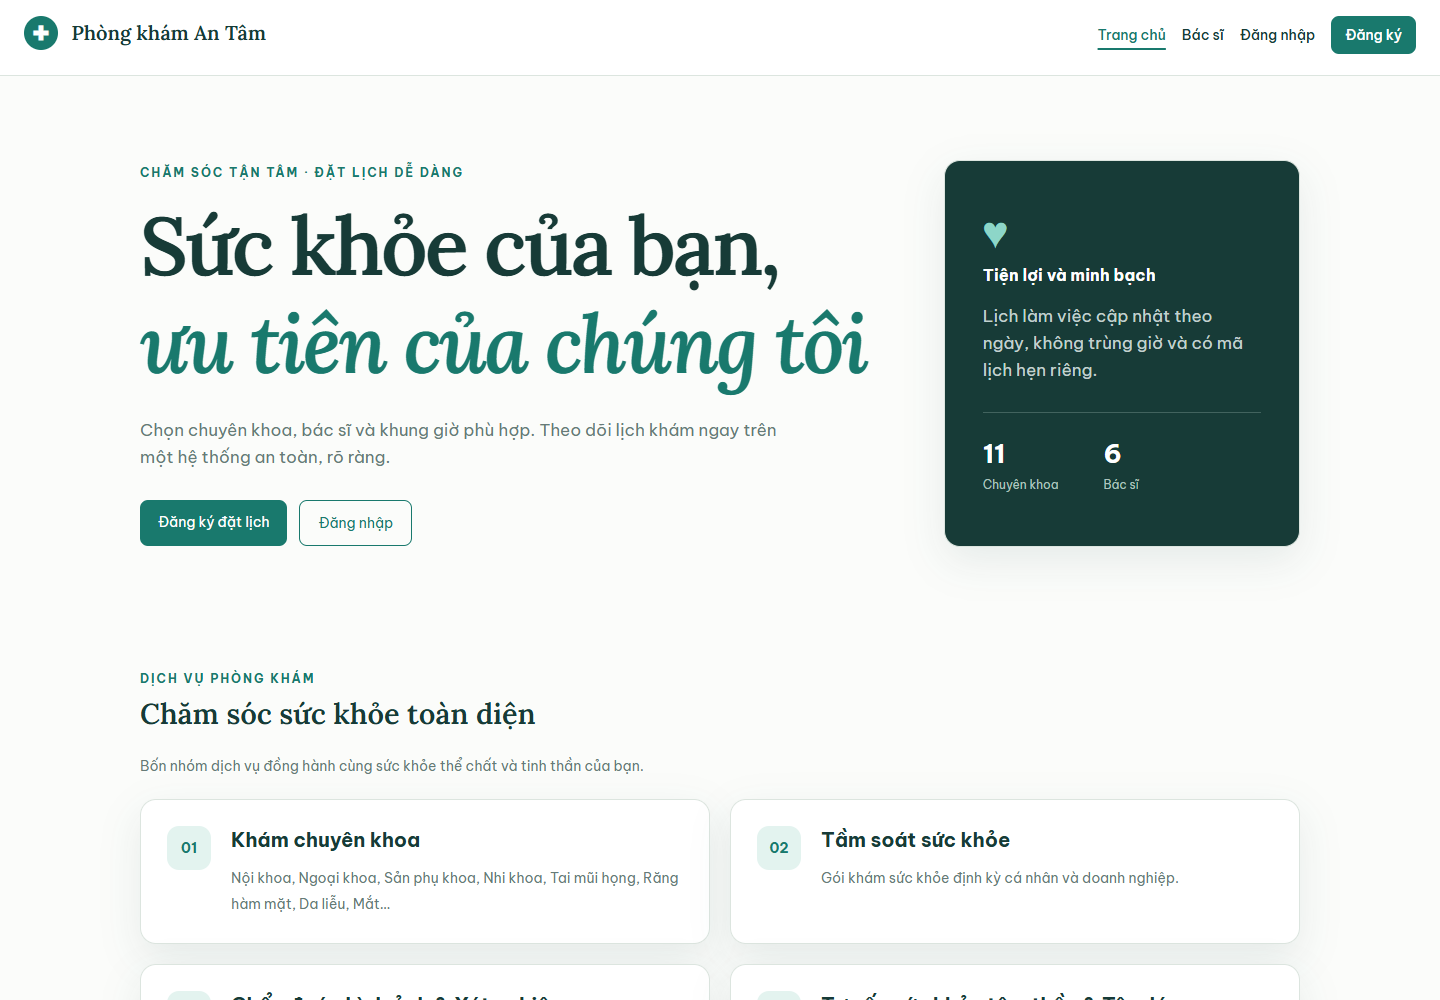
\includegraphics[width=\textwidth,height=.57\textheight,keepaspectratio]{figures/ui/home.png}\captionof{figure}{Trang chủ và nhóm dịch vụ}\end{center}
Bốn nhóm dịch vụ định hướng người dùng tới tra cứu bác sĩ và đặt lịch.\allowbreak{} Số lượng bác sĩ trên khối giới thiệu là danh sách giới hạn ở trang chủ, không phải lúc nào cũng là tổng lực lượng.\allowbreak{}

Vai trò minh họa:\allowbreak{} Công khai.\allowbreak{} Đường dẫn chức năng:\allowbreak{} /\allowbreak{}.\allowbreak{}

\clearpage

\Needspace{6\baselineskip}\subsection{Đăng nhập và hiện mật khẩu}
\begin{center}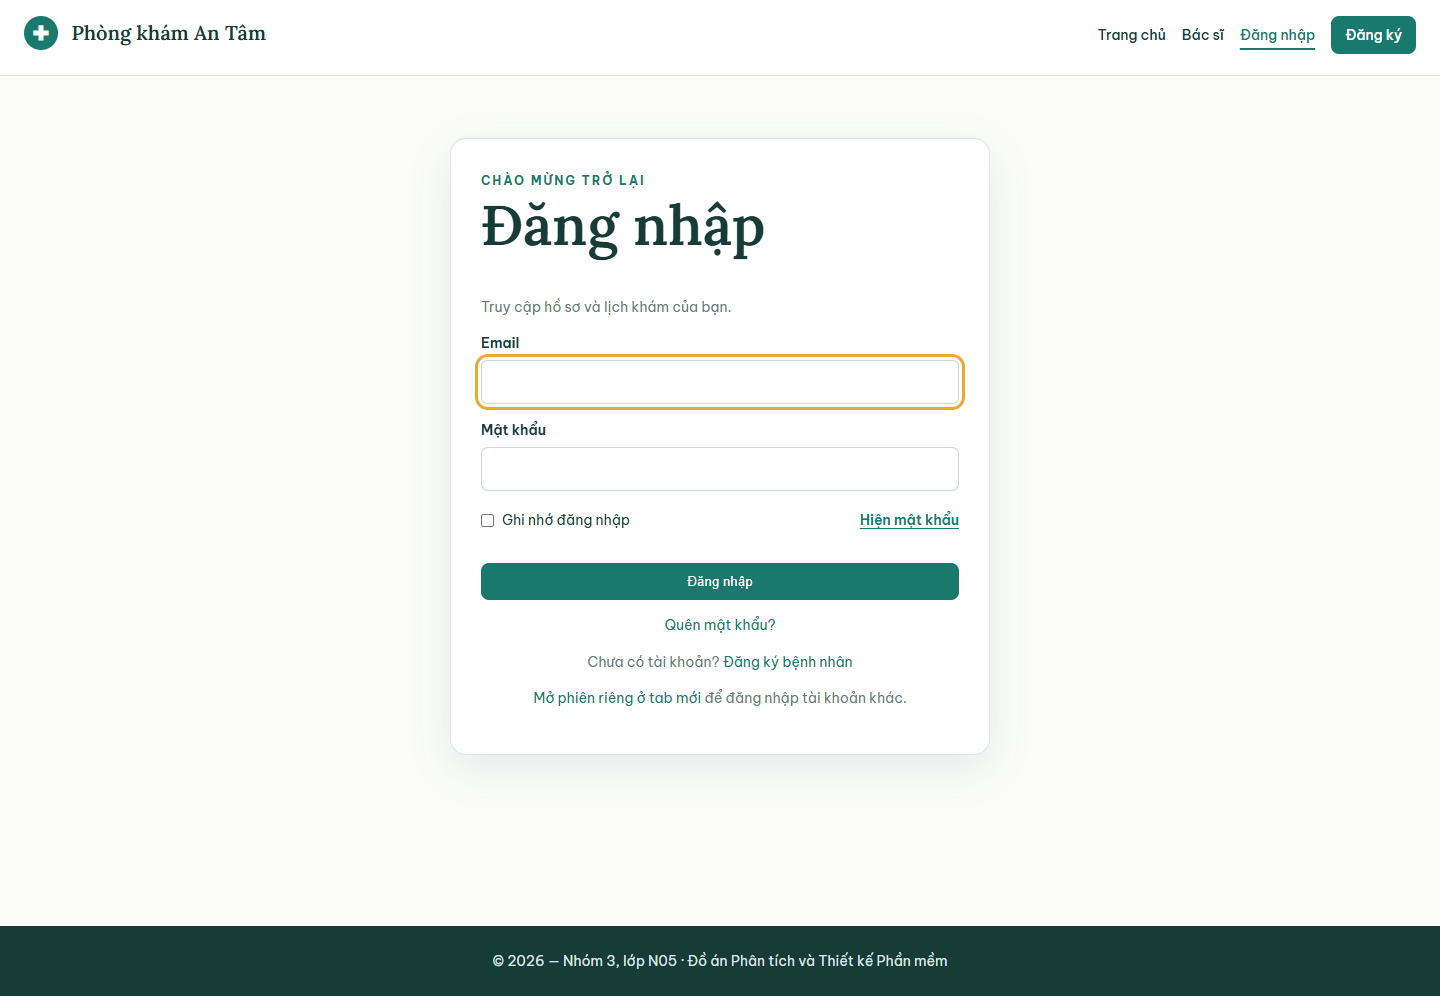
\includegraphics[width=\textwidth,height=.57\textheight,keepaspectratio]{figures/ui/login.png}\captionof{figure}{Đăng nhập và hiện mật khẩu}\end{center}
Nút Hiện mật khẩu chỉ đổi cách hiển thị input ở trình duyệt.\allowbreak{} Thông tin mật khẩu vẫn được gửi qua cơ chế form và xác thực; báo cáo không hiển thị mật khẩu tài khoản trên ảnh.\allowbreak{}

Vai trò minh họa:\allowbreak{} Công khai.\allowbreak{} Đường dẫn chức năng:\allowbreak{} /\allowbreak{}dang-nhap.\allowbreak{}

\clearpage

\Needspace{6\baselineskip}\subsection{Danh sách bác sĩ theo cơ sở và chuyên khoa}
\begin{center}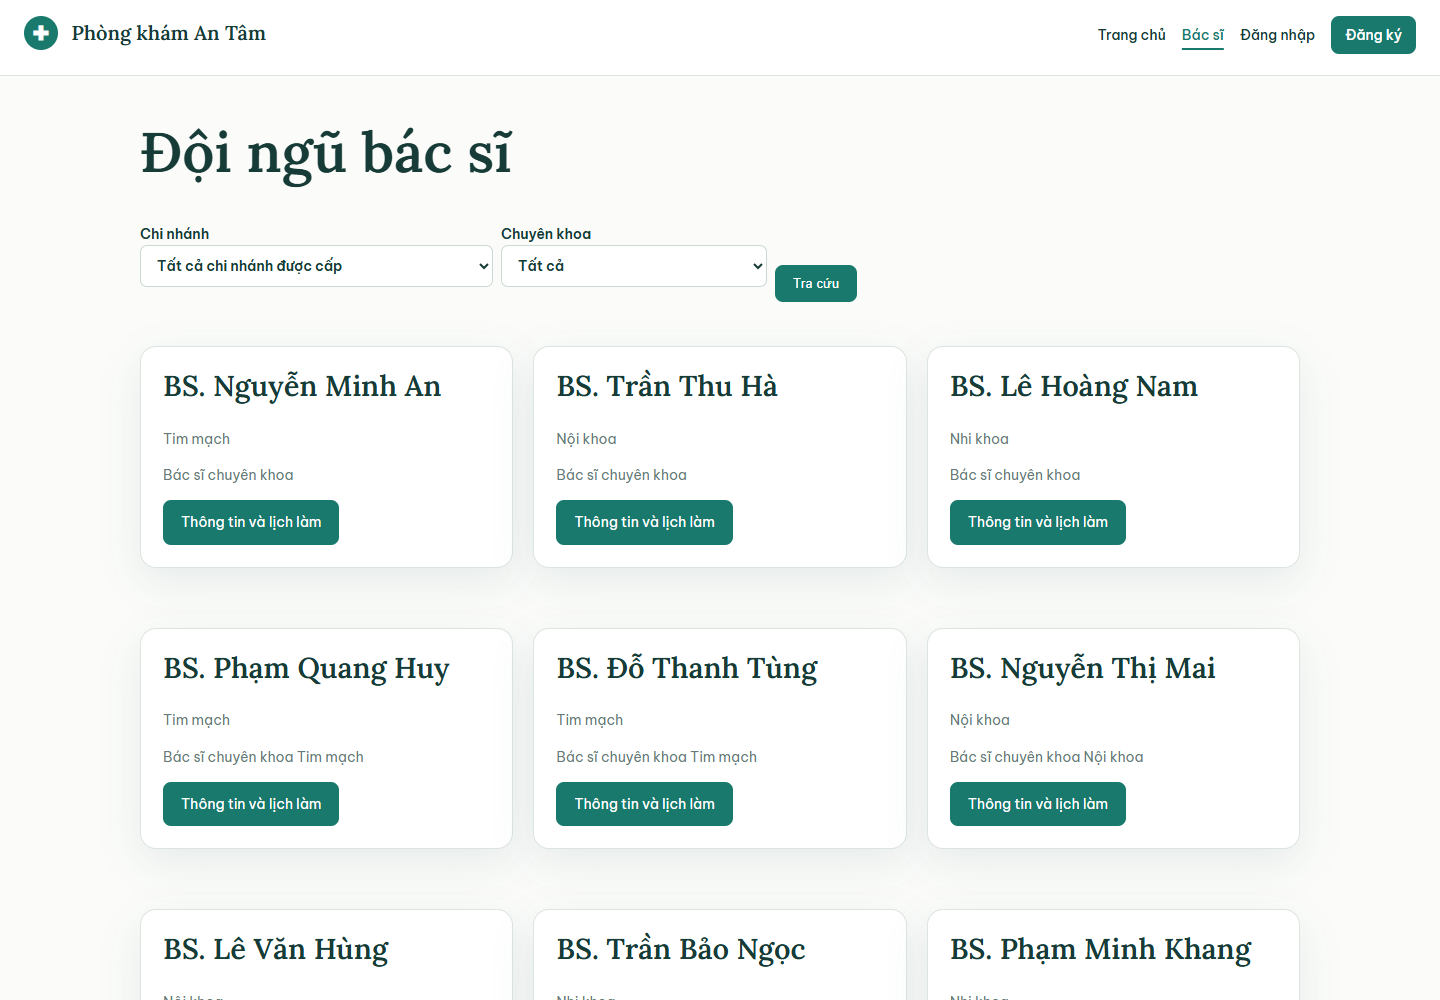
\includegraphics[width=\textwidth,height=.57\textheight,keepaspectratio]{figures/ui/doctors.png}\captionof{figure}{Danh sách bác sĩ theo cơ sở và chuyên khoa}\end{center}
Bộ lọc và phân trang giúp giới hạn danh sách, mỗi thẻ dẫn tới thông tin chi tiết.\allowbreak{} Dữ liệu nhân sự trong ảnh là bộ học tập riêng.\allowbreak{}

Vai trò minh họa:\allowbreak{} Công khai.\allowbreak{} Đường dẫn chức năng:\allowbreak{} /\allowbreak{}bac-si.\allowbreak{}

\clearpage

\Needspace{6\baselineskip}\subsection{Khôi phục mật khẩu}
\begin{center}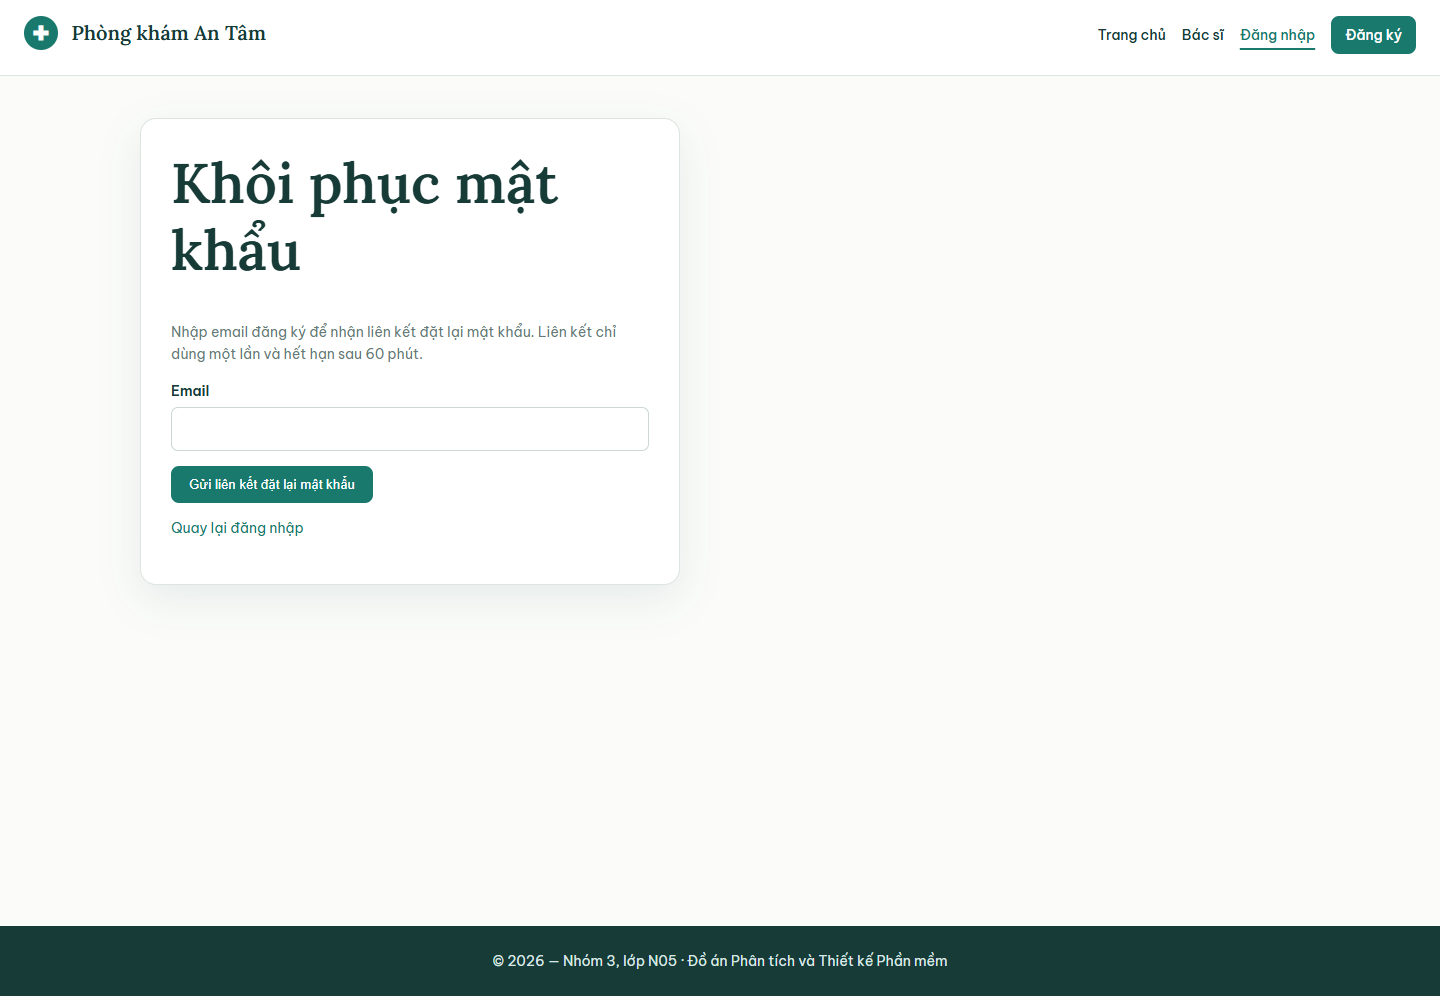
\includegraphics[width=\textwidth,height=.57\textheight,keepaspectratio]{figures/ui/forgot.png}\captionof{figure}{Khôi phục mật khẩu}\end{center}
Giới hạn tần suất giữ biểu mẫu và thời gian chờ; phản hồi gửi liên kết không tiết lộ email đã đăng ký.\allowbreak{} Ảnh không minh chứng email đã được giao tới SMTP thật.\allowbreak{}

Vai trò minh họa:\allowbreak{} Công khai.\allowbreak{} Đường dẫn chức năng:\allowbreak{} /\allowbreak{}quen-mat-khau.\allowbreak{}

\clearpage

\Needspace{6\baselineskip}\subsection{Đặt lịch theo ca và giờ trống}
\begin{center}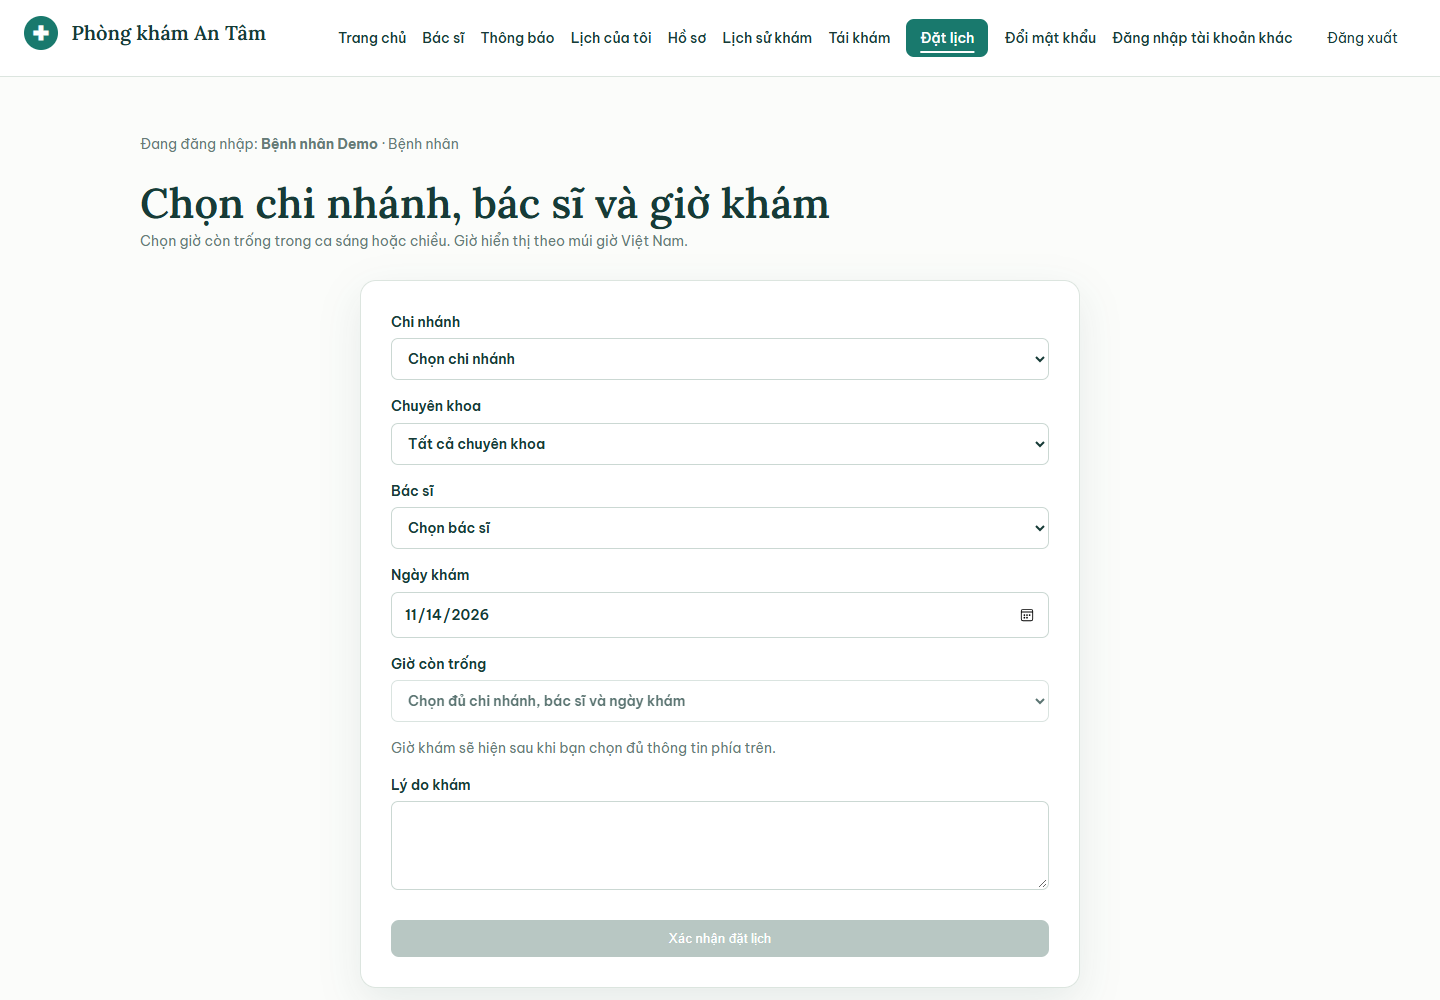
\includegraphics[width=\textwidth,height=.57\textheight,keepaspectratio]{figures/ui/booking.png}\captionof{figure}{Đặt lịch theo ca và giờ trống}\end{center}
Chi nhánh, chuyên khoa, bác sĩ và ngày điều khiển truy vấn giờ khả dụng.\allowbreak{} Giờ trên giao diện chỉ là gợi ý; service khóa và kiểm lại khi xác nhận đặt.\allowbreak{}

Vai trò minh họa:\allowbreak{} Bệnh nhân.\allowbreak{} Đường dẫn chức năng:\allowbreak{} /\allowbreak{}lich-kham/\allowbreak{}dat-lich.\allowbreak{}

\clearpage

\Needspace{6\baselineskip}\subsection{Lịch hẹn của bệnh nhân}
\begin{center}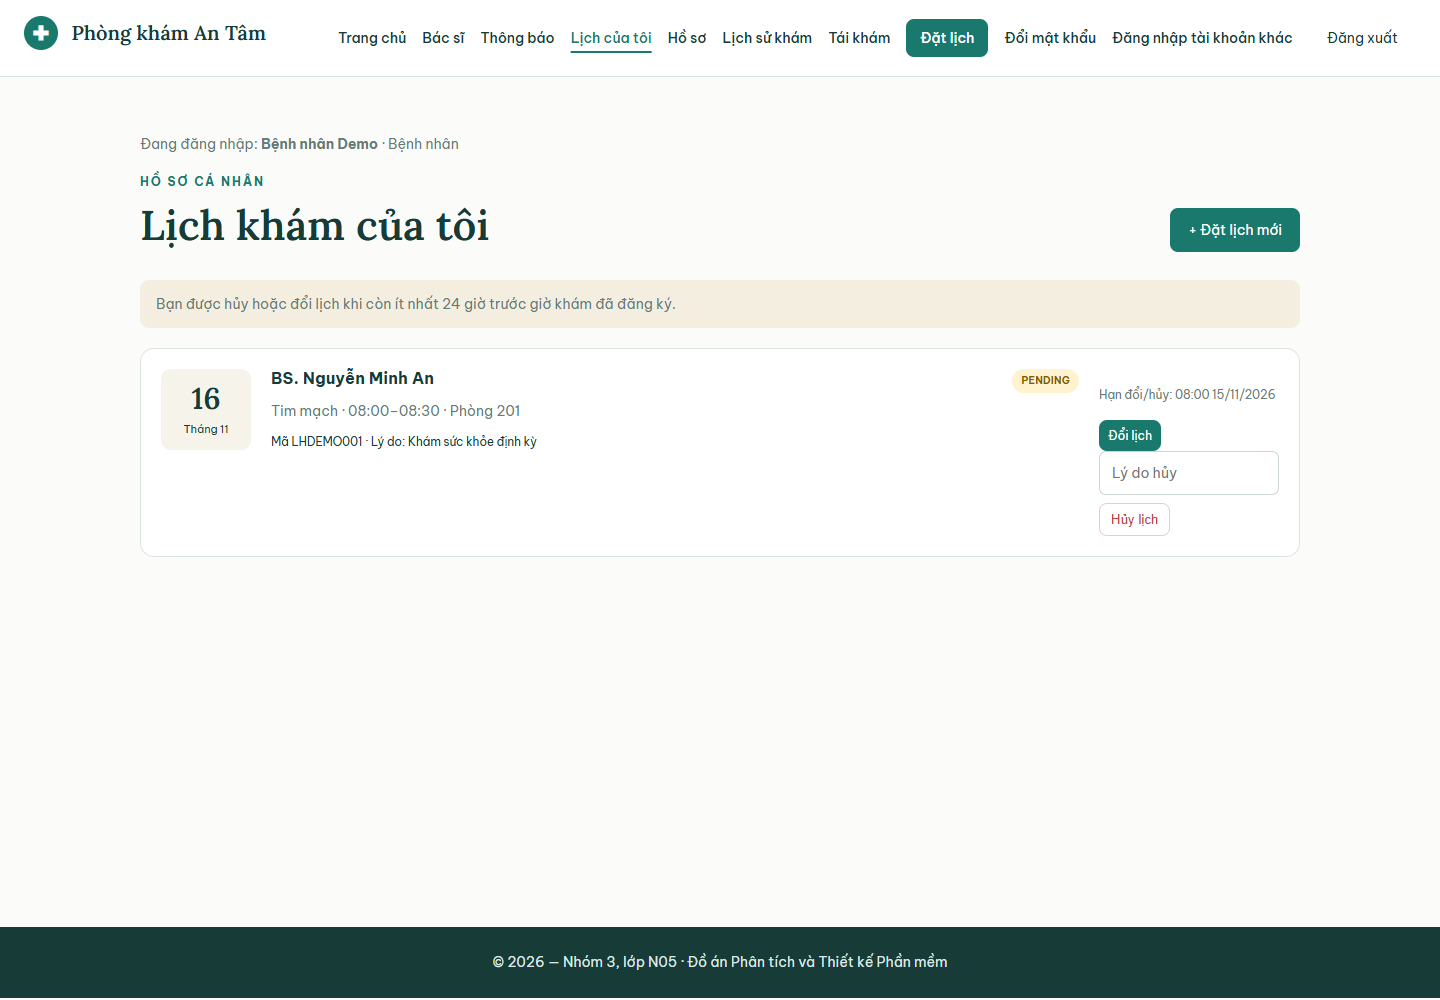
\includegraphics[width=\textwidth,height=.57\textheight,keepaspectratio]{figures/ui/appointments.png}\captionof{figure}{Lịch hẹn của bệnh nhân}\end{center}
PENDING là Chờ xác nhận.\allowbreak{} Hạn đổi/\allowbreak{}hủy lấy từ giờ đã đăng ký trừ ngưỡng cấu hình.\allowbreak{} Lịch bị chặn vẫn được giữ và phản hồi bằng thông báo nghiệp vụ.\allowbreak{}

Vai trò minh họa:\allowbreak{} Bệnh nhân.\allowbreak{} Đường dẫn chức năng:\allowbreak{} /\allowbreak{}lich-kham.\allowbreak{}

\clearpage

\Needspace{6\baselineskip}\subsection{Lịch của tôi và đăng ký ca bác sĩ}
\begin{center}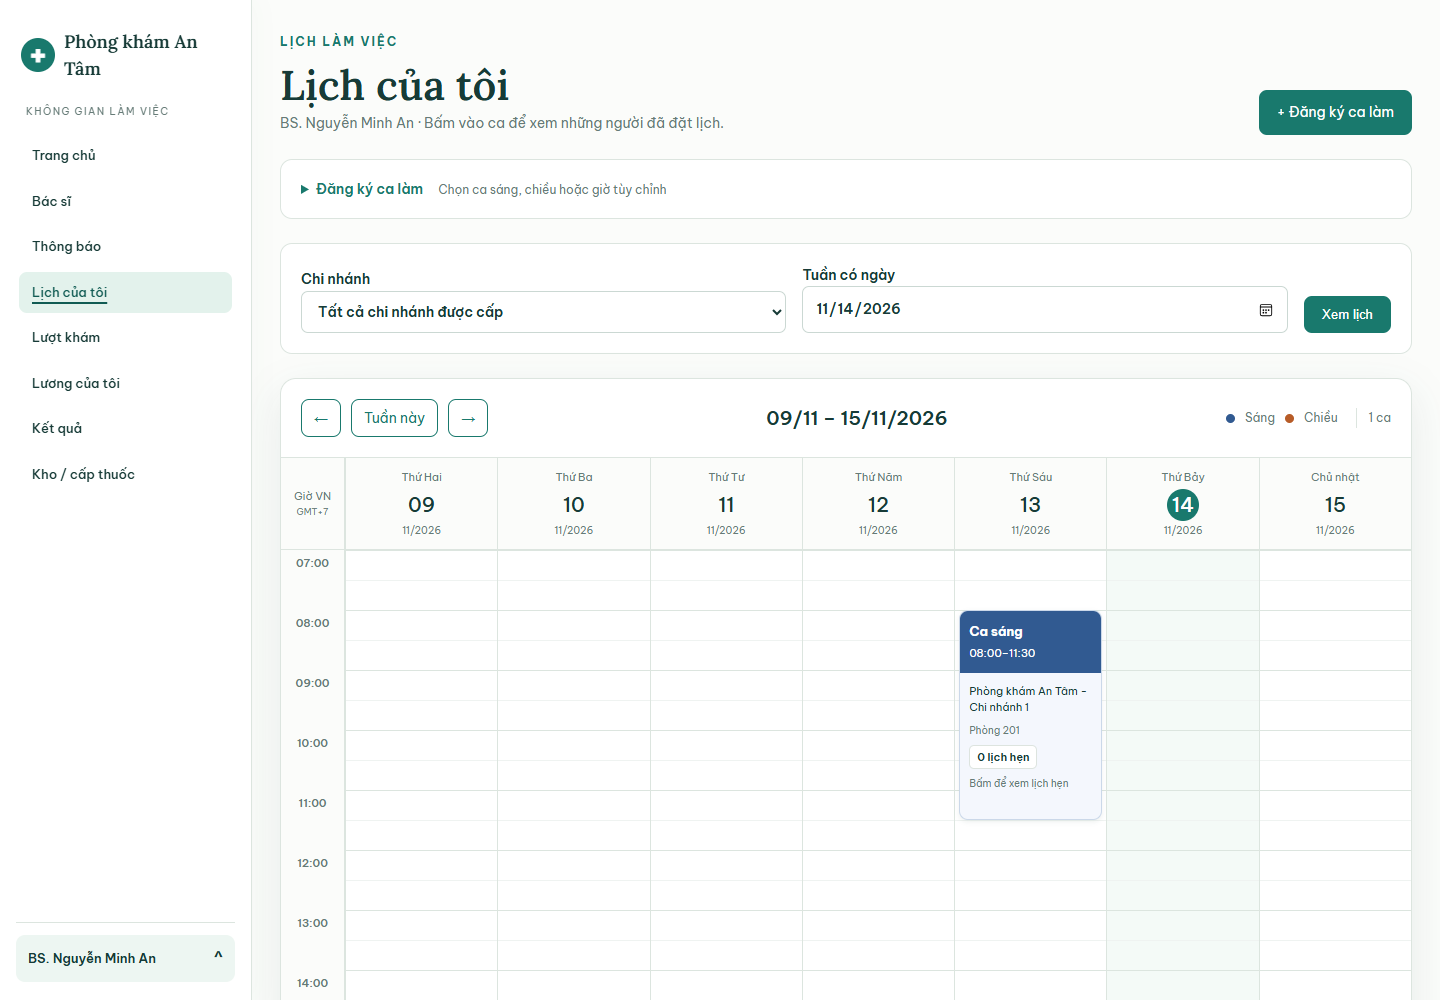
\includegraphics[width=\textwidth,height=.57\textheight,keepaspectratio]{figures/ui/doctor-calendar.png}\captionof{figure}{Lịch của tôi và đăng ký ca bác sĩ}\end{center}
Lịch tuần chỉ có ca của bác sĩ hiện tại.\allowbreak{} Nhấn ca mới tải bệnh nhân; phần đăng ký ca ở cùng mục, không tạo một menu điều hướng mới.\allowbreak{}

Vai trò minh họa:\allowbreak{} Bác sĩ.\allowbreak{} Đường dẫn chức năng:\allowbreak{} /\allowbreak{}nhan-vien/\allowbreak{}lich-hen.\allowbreak{}

\clearpage

\Needspace{6\baselineskip}\subsection{Danh sách lượt khám được giao}
\begin{center}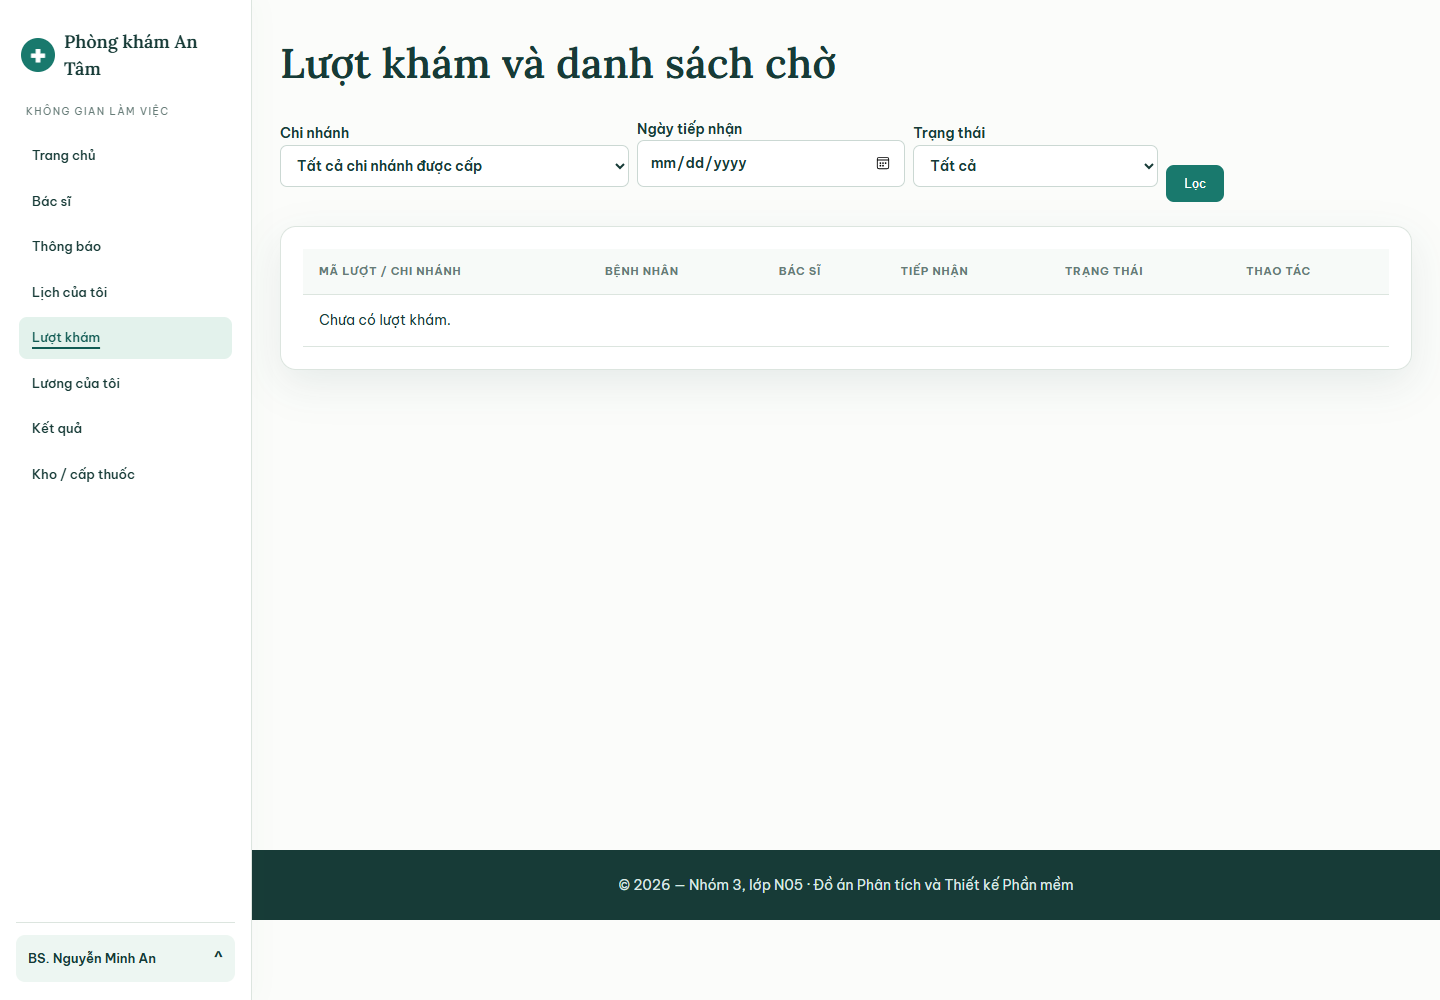
\includegraphics[width=\textwidth,height=.57\textheight,keepaspectratio]{figures/ui/visits.png}\captionof{figure}{Danh sách lượt khám được giao}\end{center}
Màn hình lọc theo người được giao và quyền cơ sở.\allowbreak{} Trong bộ minh họa chưa tiếp nhận lượt nên trạng thái rỗng là hợp lệ, không phải lỗi tải dữ liệu.\allowbreak{}

Vai trò minh họa:\allowbreak{} Bác sĩ.\allowbreak{} Đường dẫn chức năng:\allowbreak{} /\allowbreak{}luot-kham.\allowbreak{}

\clearpage

\Needspace{6\baselineskip}\subsection{Lương cá nhân chỉ đọc}
\begin{center}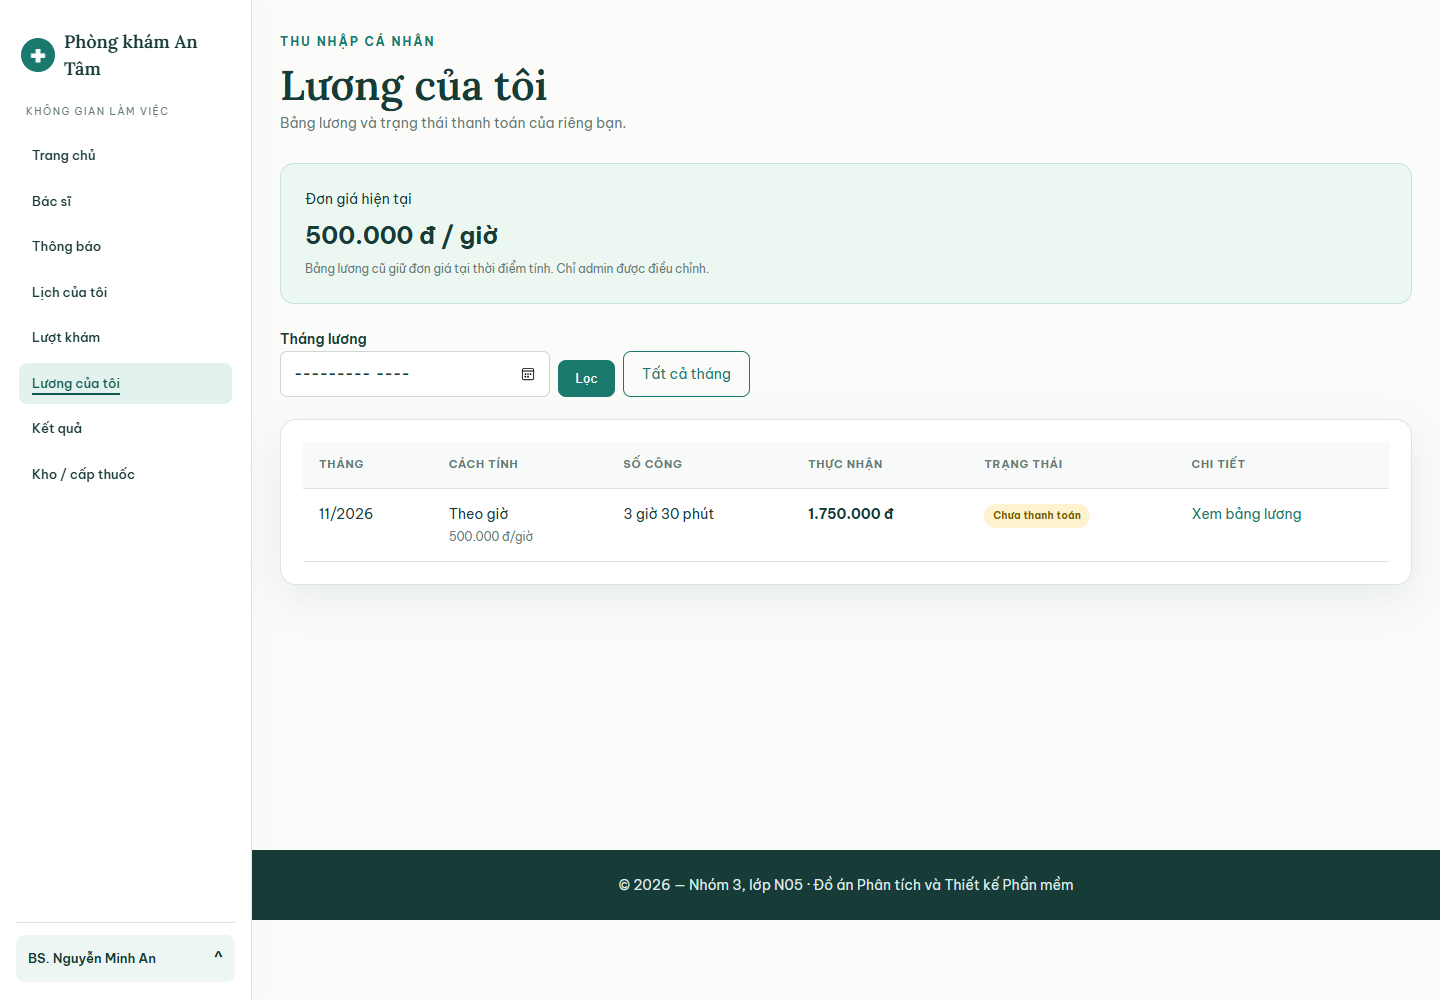
\includegraphics[width=\textwidth,height=.57\textheight,keepaspectratio]{figures/ui/my-payroll.png}\captionof{figure}{Lương cá nhân chỉ đọc}\end{center}
Bác sĩ xem đúng bảng thuộc tài khoản mình; nguồn giờ và số tiền mẫu dùng để minh họa.\allowbreak{} Nhân viên không có form sửa đơn giá hoặc ghi thanh toán.\allowbreak{}

Vai trò minh họa:\allowbreak{} Bác sĩ.\allowbreak{} Đường dẫn chức năng:\allowbreak{} /\allowbreak{}luong-cua-toi.\allowbreak{}

\clearpage

\Needspace{6\baselineskip}\subsection{Thông báo và thao tác xác nhận của lễ tân}
\begin{center}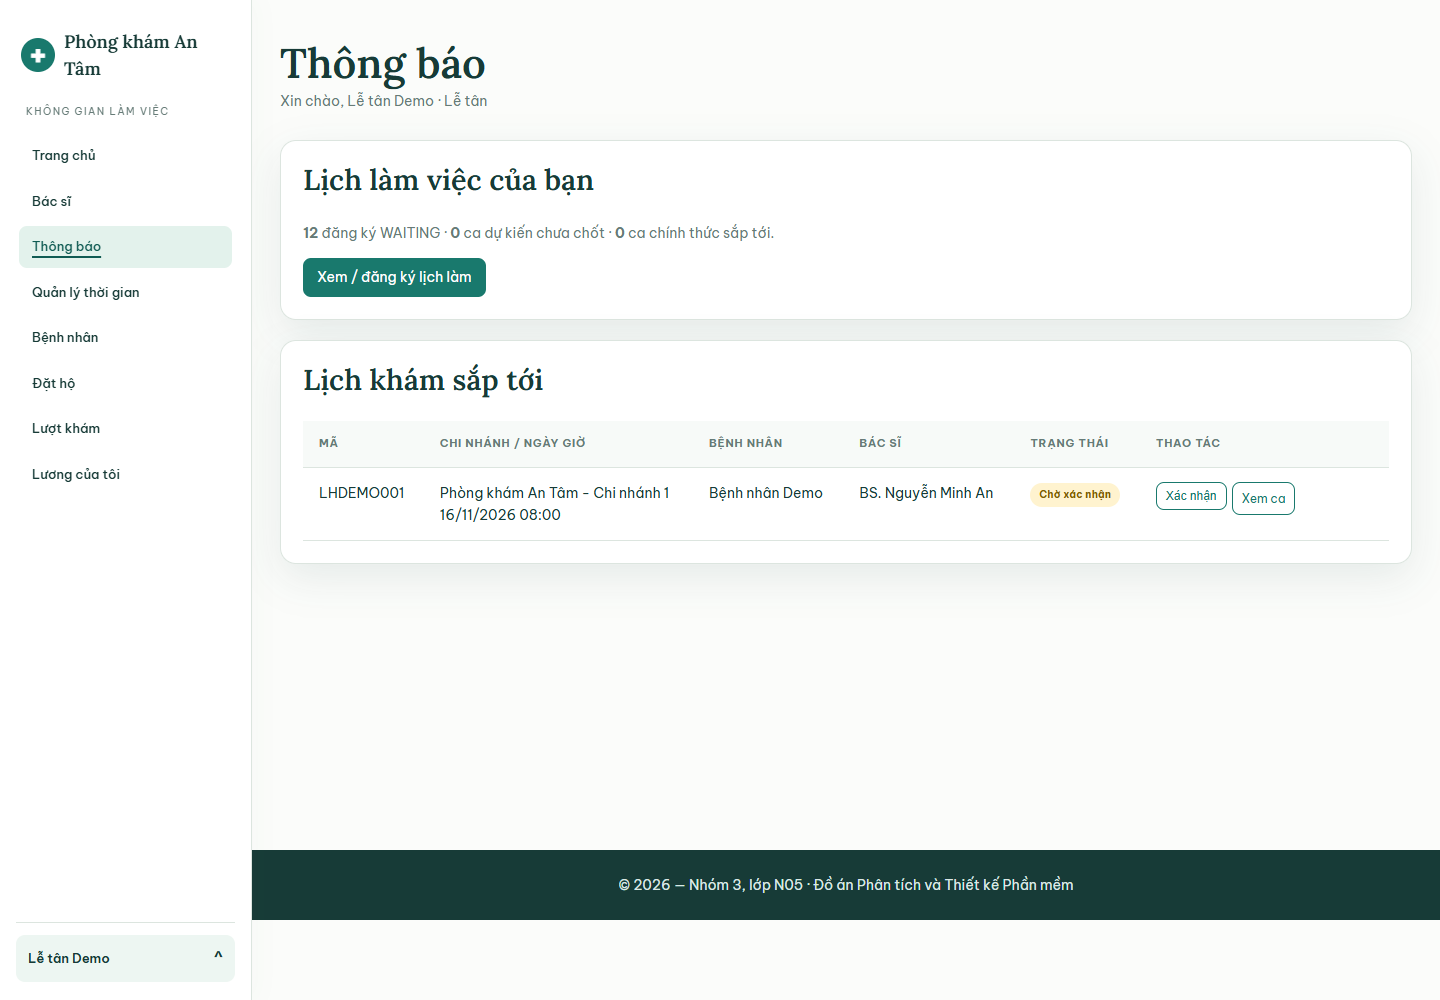
\includegraphics[width=\textwidth,height=.57\textheight,keepaspectratio]{figures/ui/reception-dashboard.png}\captionof{figure}{Thông báo và thao tác xác nhận của lễ tân}\end{center}
Nút xác nhận/\allowbreak{}tiếp nhận phụ thuộc trạng thái và ngày khám.\allowbreak{} Thông tin tài khoản nằm ở cuối thanh bên; nhấn tên mới mở các hành động tài khoản.\allowbreak{}

Vai trò minh họa:\allowbreak{} Lễ tân.\allowbreak{} Đường dẫn chức năng:\allowbreak{} /\allowbreak{}bang-dieu-khien.\allowbreak{}

\clearpage

\Needspace{6\baselineskip}\subsection{Nguyện vọng lịch làm nhân viên}
\begin{center}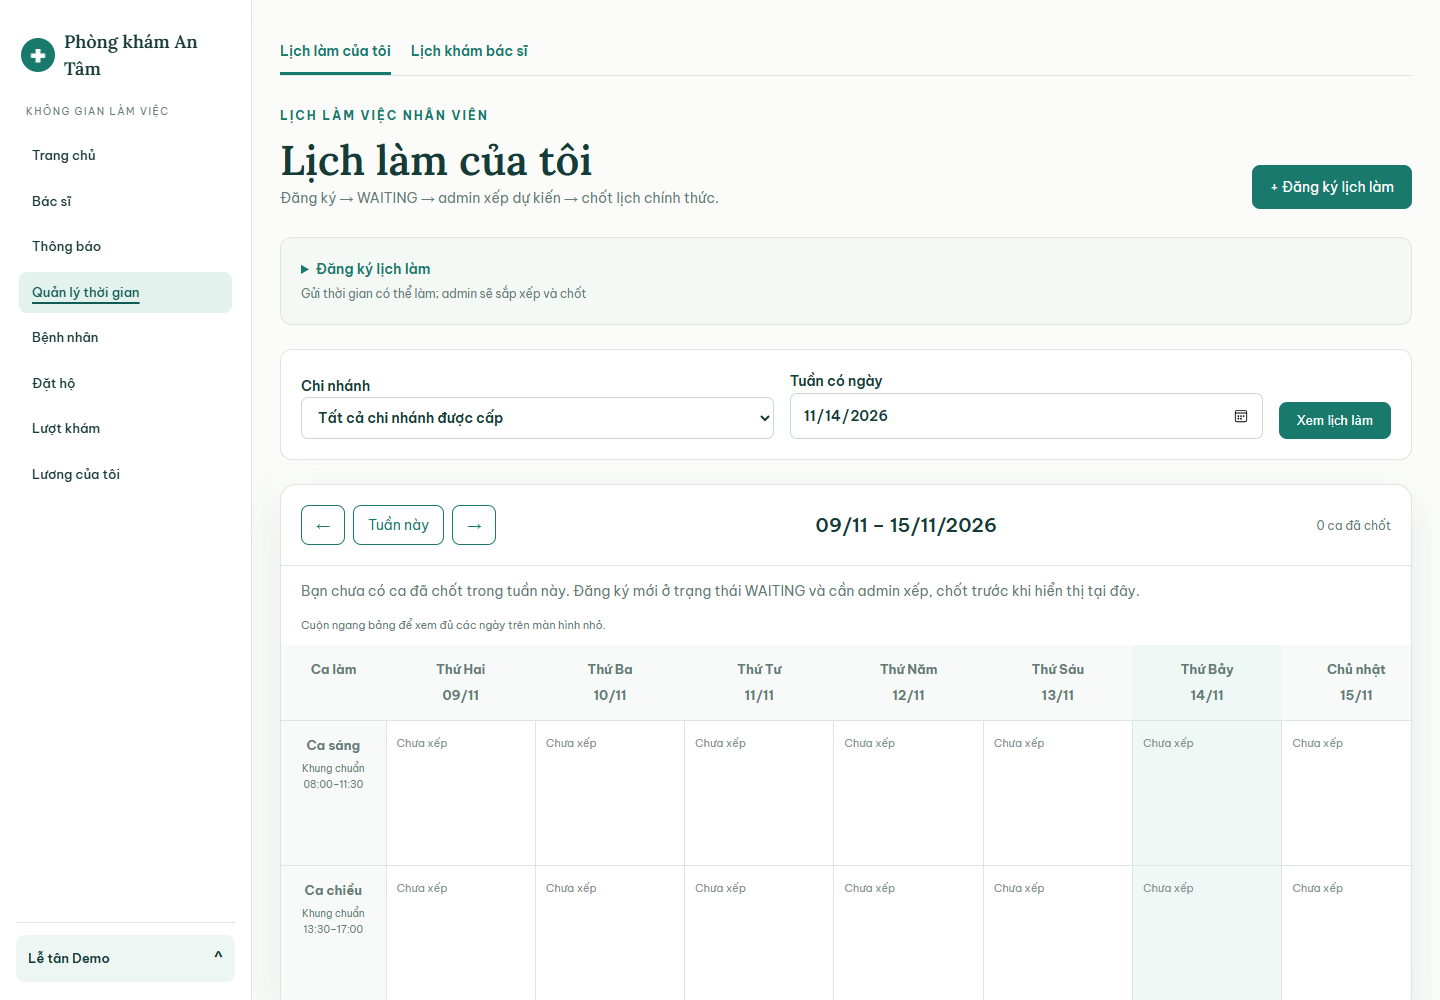
\includegraphics[width=\textwidth,height=.57\textheight,keepaspectratio]{figures/ui/employee-roster.png}\captionof{figure}{Nguyện vọng lịch làm nhân viên}\end{center}
WAITING nghĩa là chờ xếp, ARRANGED là có phương án dự kiến.\allowbreak{} Chỉ ca đã chốt được xem như lịch chính thức; ảnh có đăng ký mẫu riêng.\allowbreak{}

Vai trò minh họa:\allowbreak{} Lễ tân.\allowbreak{} Đường dẫn chức năng:\allowbreak{} /\allowbreak{}nhan-vien/\allowbreak{}lich-lam-viec.\allowbreak{}

\clearpage

\Needspace{6\baselineskip}\subsection{Xếp lịch nhân viên chia bảng theo cơ sở}
\begin{center}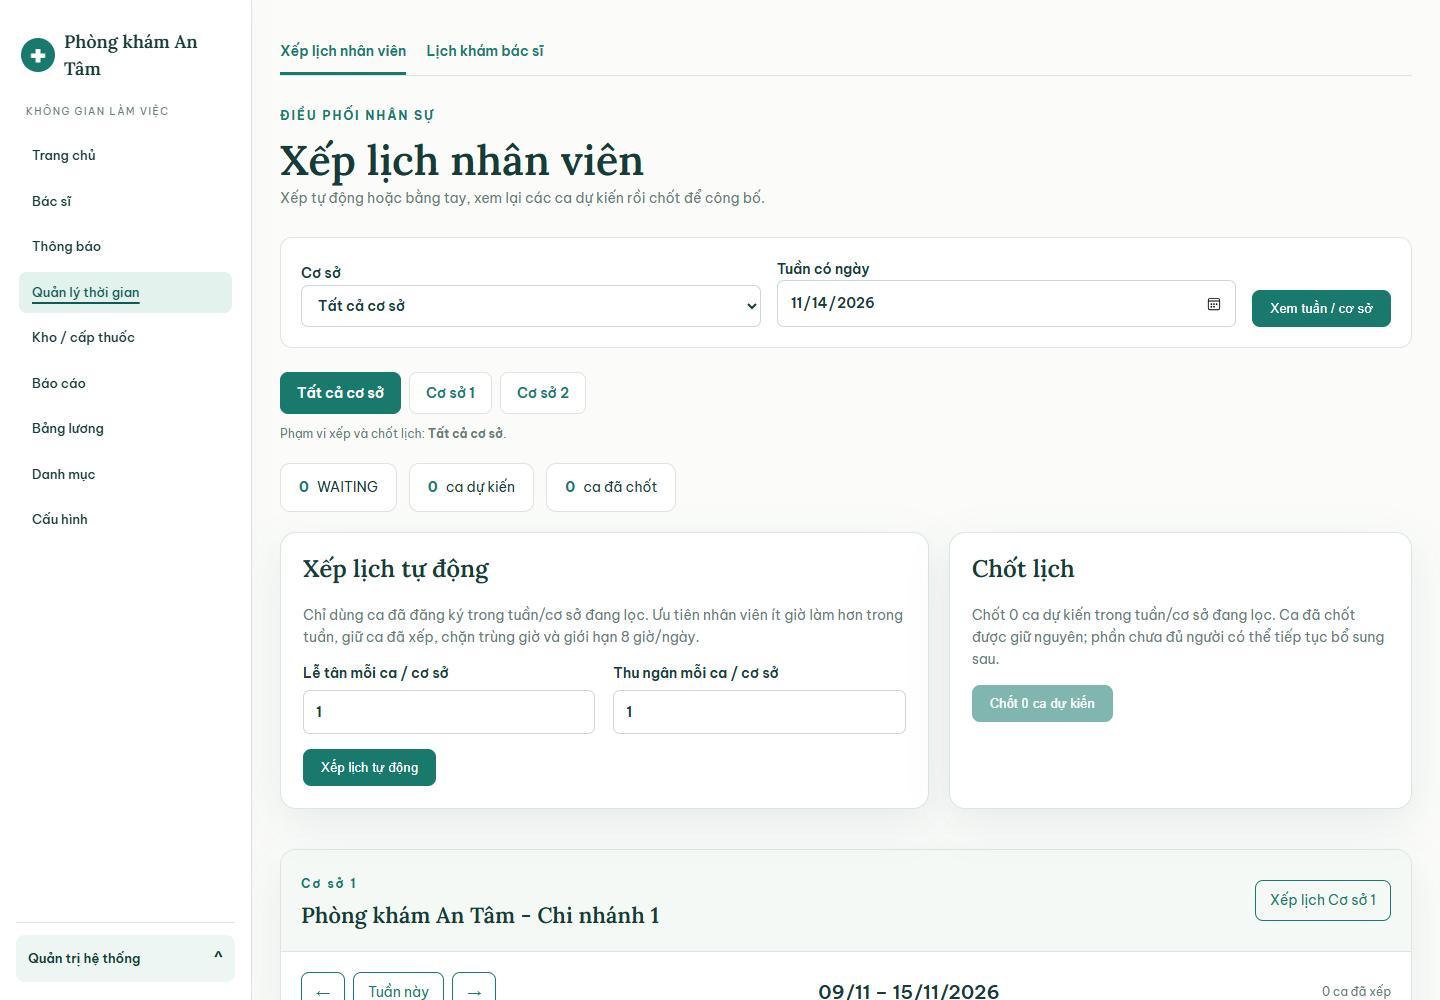
\includegraphics[width=\textwidth,height=.57\textheight,keepaspectratio]{figures/ui/admin-roster.png}\captionof{figure}{Xếp lịch nhân viên chia bảng theo cơ sở}\end{center}
Nút cơ sở và các bảng giúp rà soát người làm theo địa điểm.\allowbreak{} Xếp tự động chỉ tạo dự kiến; admin cần xem phạm vi tuần/\allowbreak{}cơ sở trước khi chốt.\allowbreak{}

Vai trò minh họa:\allowbreak{} Quản trị viên.\allowbreak{} Đường dẫn chức năng:\allowbreak{} /\allowbreak{}quan-tri/\allowbreak{}lich-nhan-vien.\allowbreak{}

\clearpage

\Needspace{6\baselineskip}\subsection{Quản trị bảng lương và đơn giá}
\begin{center}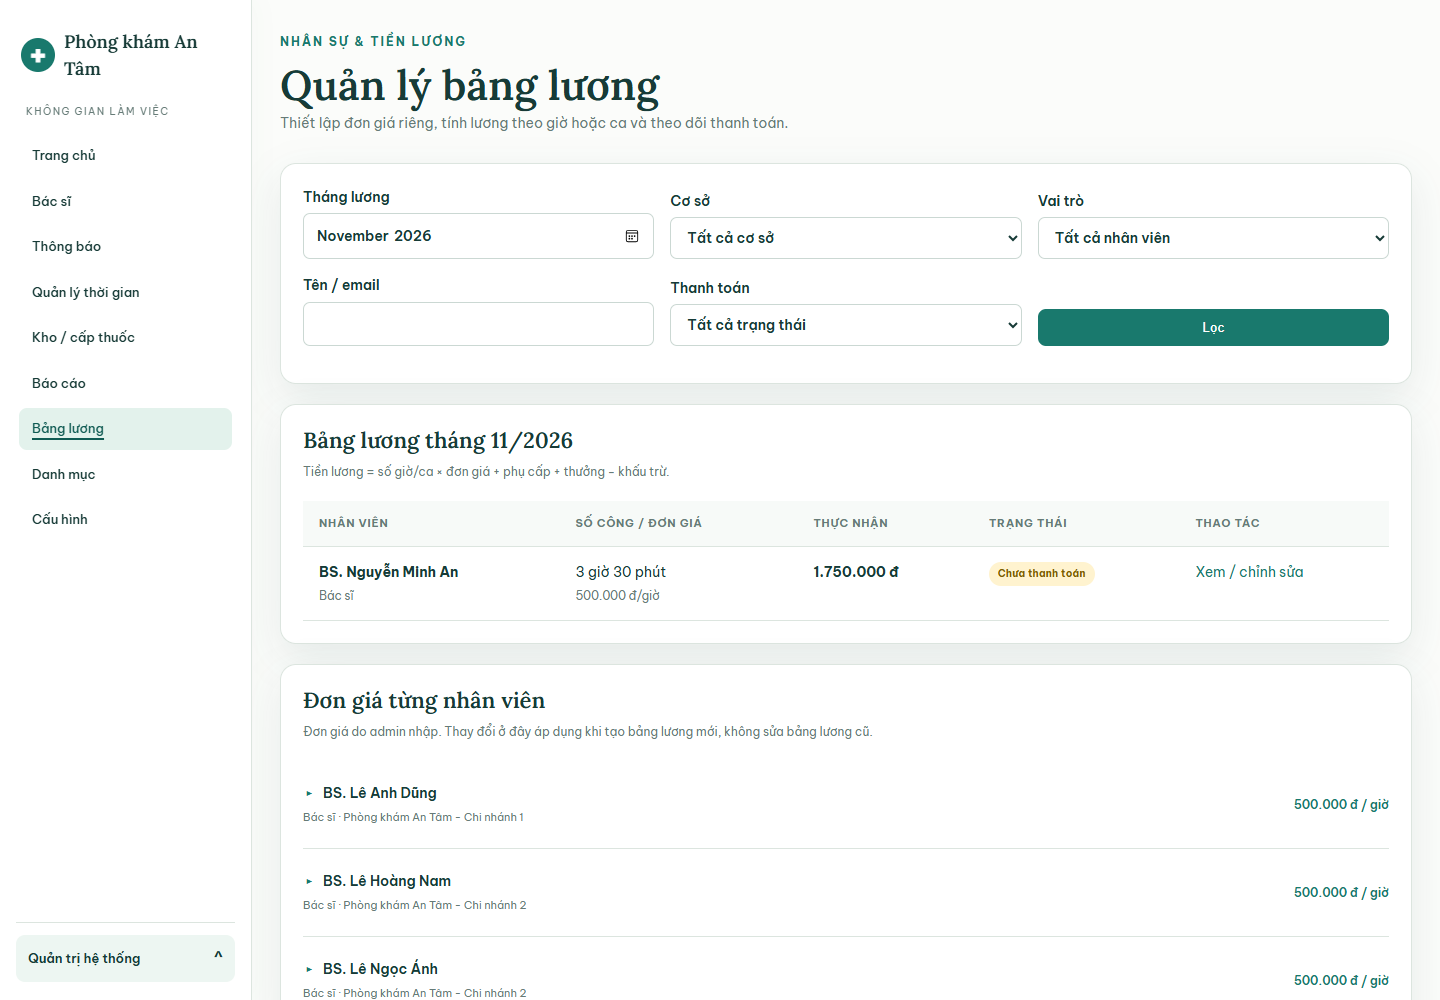
\includegraphics[width=\textwidth,height=.57\textheight,keepaspectratio]{figures/ui/admin-payroll.png}\captionof{figure}{Quản trị bảng lương và đơn giá}\end{center}
Bộ lọc tháng/\allowbreak{}cơ sở/\allowbreak{}vai trò và trạng thái hỗ trợ tìm bảng.\allowbreak{} Mũi tên đơn giá tăng giảm bước 1.\allowbreak{}000 VND, đơn giá của từng người lưu riêng.\allowbreak{}

Vai trò minh họa:\allowbreak{} Quản trị viên.\allowbreak{} Đường dẫn chức năng:\allowbreak{} /\allowbreak{}quan-tri/\allowbreak{}bang-luong.\allowbreak{}

\clearpage

\Needspace{6\baselineskip}\subsection{Tồn thuốc theo cơ sở và lô}
\begin{center}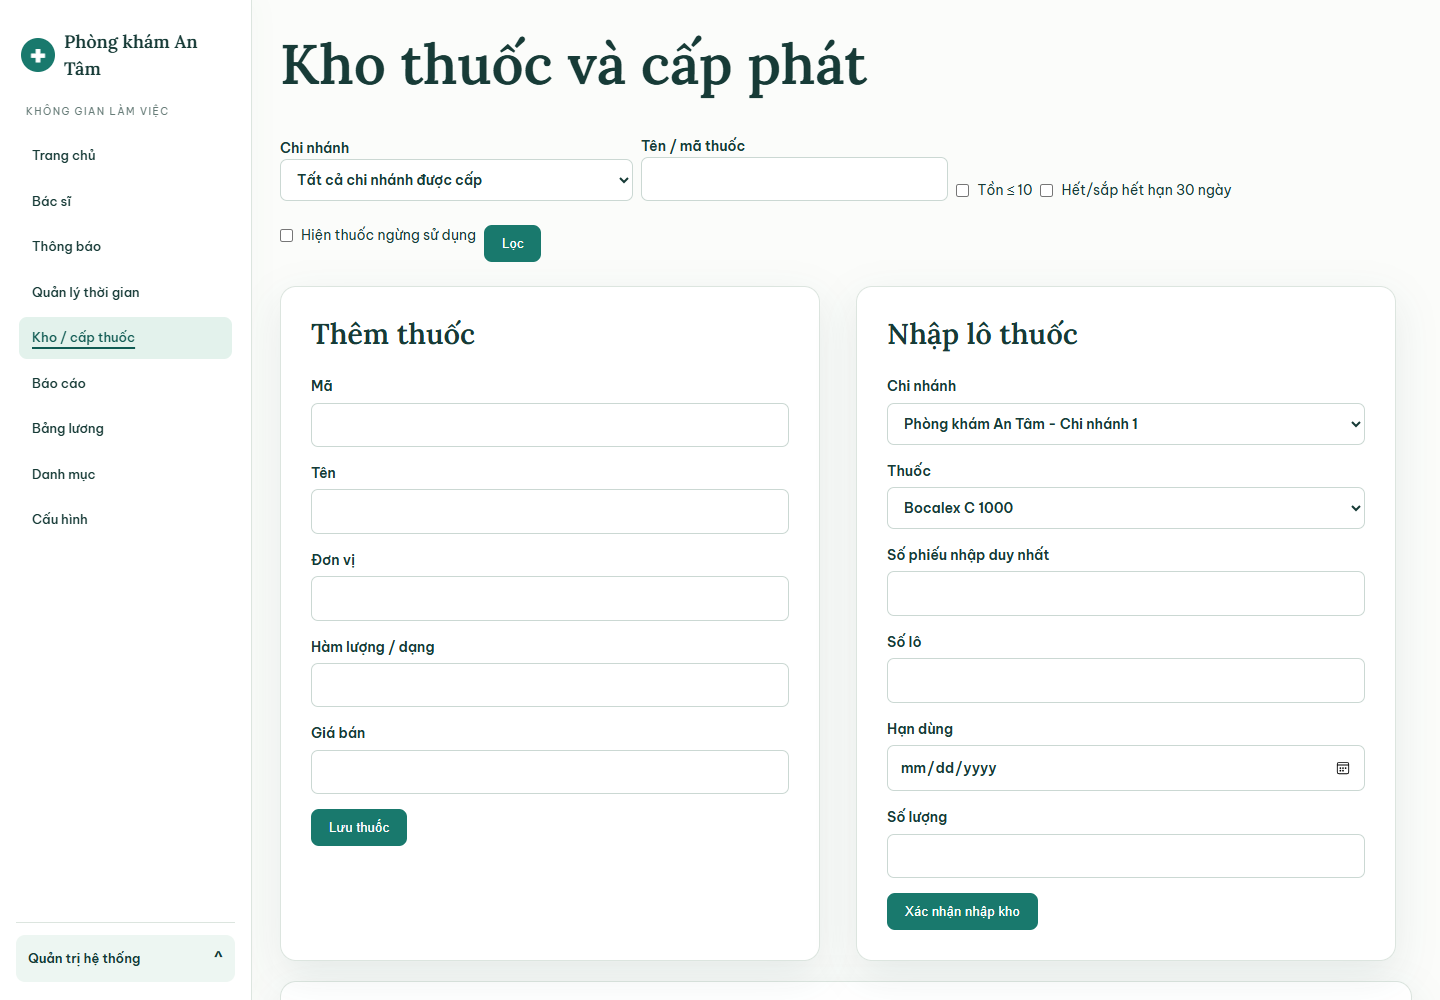
\includegraphics[width=\textwidth,height=.57\textheight,keepaspectratio]{figures/ui/inventory.png}\captionof{figure}{Tồn thuốc theo cơ sở và lô}\end{center}
Tồn và hạn dùng trong ảnh thuộc bộ dữ liệu học tập, không phải dữ liệu kiểm kê của nhà thuốc thật.\allowbreak{} Điều chỉnh cần chứng từ/\allowbreak{}lý do; cấp phát kiểm quyền chuyên biệt.\allowbreak{}

Vai trò minh họa:\allowbreak{} Quản trị viên.\allowbreak{} Đường dẫn chức năng:\allowbreak{} /\allowbreak{}kho.\allowbreak{}

\clearpage

\Needspace{6\baselineskip}\subsection{Cấu hình cơ sở, nhân sự và tích hợp}
\begin{center}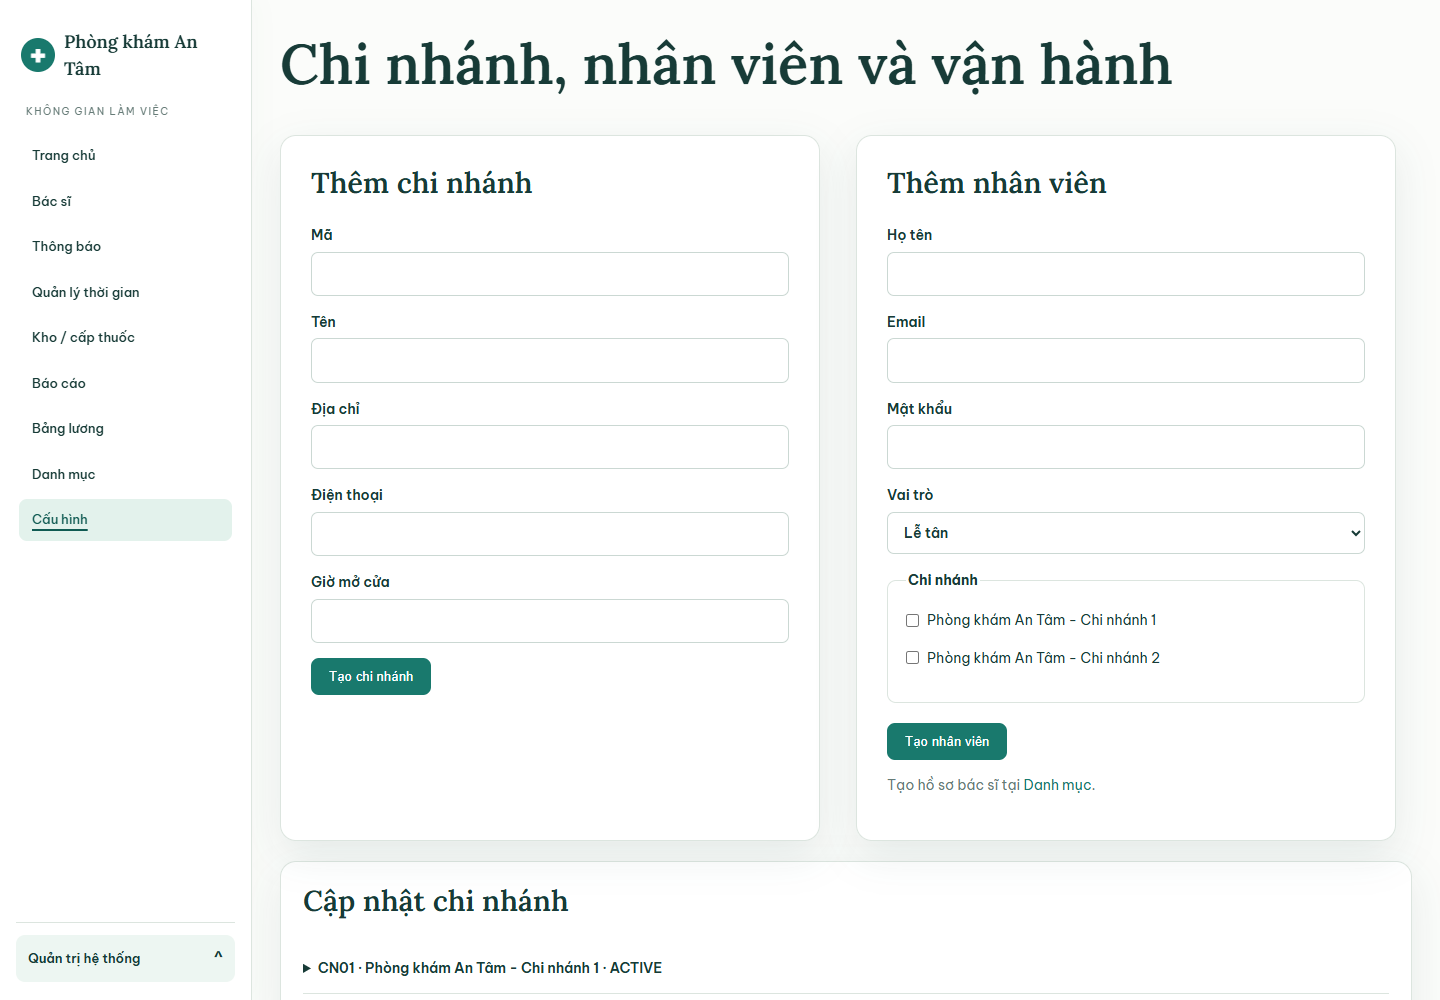
\includegraphics[width=\textwidth,height=.57\textheight,keepaspectratio]{figures/ui/settings.png}\captionof{figure}{Cấu hình cơ sở, nhân sự và tích hợp}\end{center}
Phân công cơ sở và quyền bổ sung ảnh hưởng trực tiếp phạm vi dữ liệu.\allowbreak{} Khối LIS/\allowbreak{}Device là đăng ký nguồn thử nghiệm; outbox hiển thị trạng thái gửi nền.\allowbreak{}

Vai trò minh họa:\allowbreak{} Quản trị viên.\allowbreak{} Đường dẫn chức năng:\allowbreak{} /\allowbreak{}quan-tri/\allowbreak{}cau-hinh.\allowbreak{}

\clearpage

\Needspace{6\baselineskip}\subsection{Báo cáo nghiệp vụ theo quyền}
\begin{center}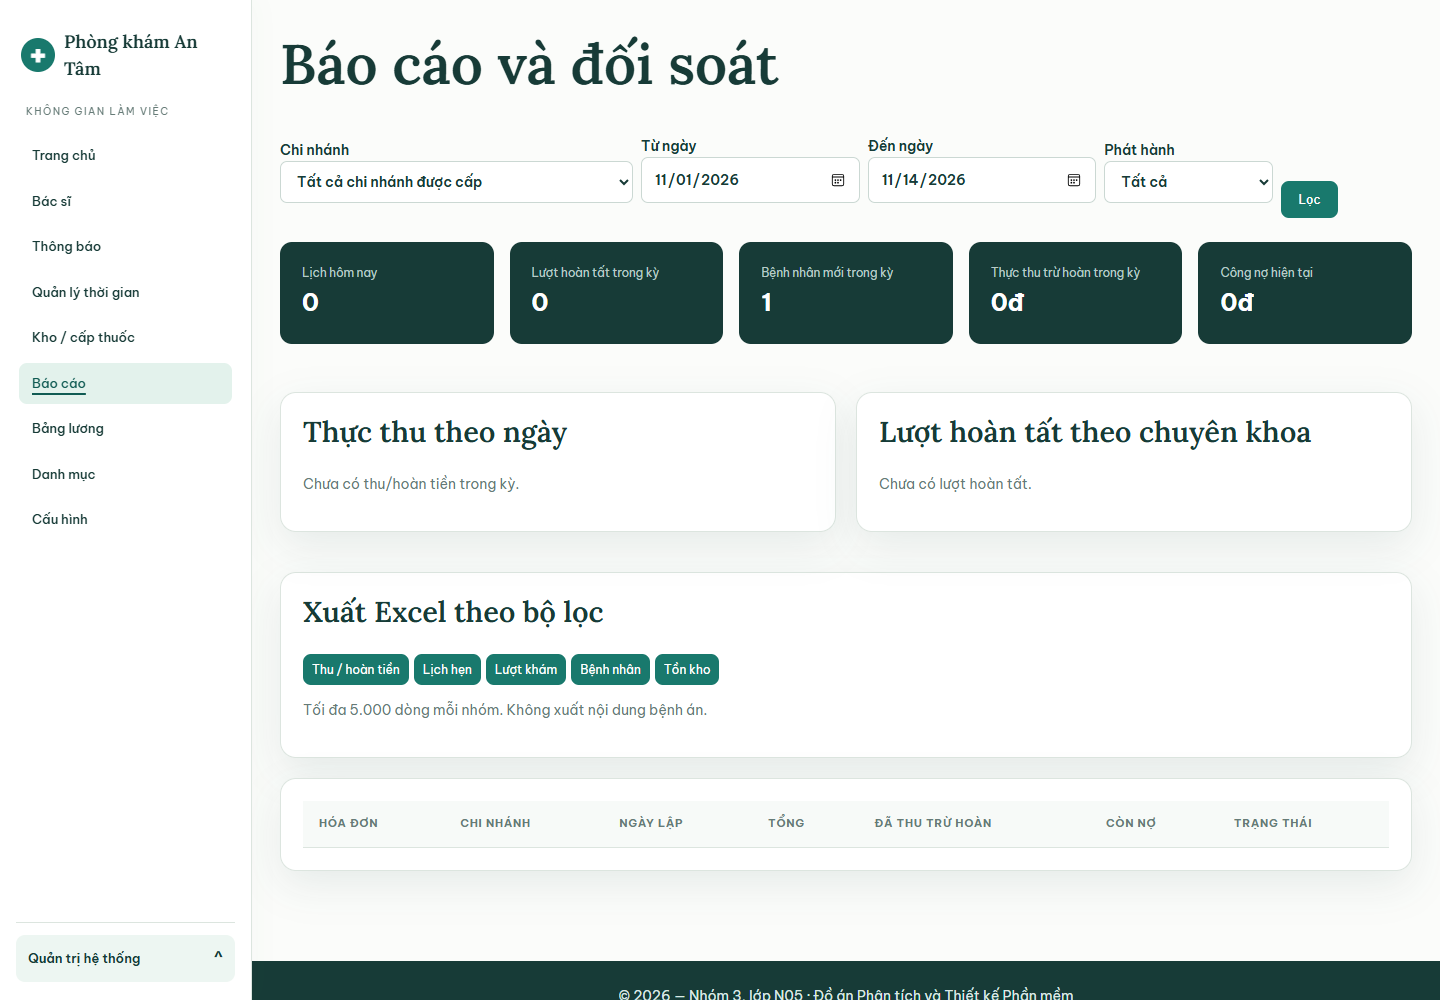
\includegraphics[width=\textwidth,height=.57\textheight,keepaspectratio]{figures/ui/reports.png}\captionof{figure}{Báo cáo nghiệp vụ theo quyền}\end{center}
Doanh thu thu thực tế trừ hoàn tiền khác tổng giá trị hóa đơn phát hành.\allowbreak{} Dữ liệu rỗng hoặc nhỏ trong ảnh là dữ liệu demo, không được dùng đánh giá hiệu quả vận hành.\allowbreak{}

Vai trò minh họa:\allowbreak{} Quản trị viên.\allowbreak{} Đường dẫn chức năng:\allowbreak{} /\allowbreak{}bao-cao.\allowbreak{}

\clearpage

\section{Kết quả chạy kiểm thử tại mốc báo cáo}
Lệnh chạy:\allowbreak{} DB\_\allowbreak{}CONNECTION=sqlite, DB\_\allowbreak{}DATABASE=:\allowbreak{}memory:\allowbreak{}, .\allowbreak{}/\allowbreak{}test.\allowbreak{}ps1 --log-junit .\allowbreak{}.\allowbreak{}.\allowbreak{} .\allowbreak{} Lần chạy ghi nhận 109 test, 2807 assertion; không có failure, error hoặc skipped trong JUnit.\allowbreak{} Thời gian và bộ nhớ dưới đây chỉ mô tả một lần chạy chức năng, không phải benchmark ứng dụng.\allowbreak{}


{\small\setlength{\tabcolsep}{3pt}\renewcommand{\arraystretch}{1.12}
\begin{longtable}{@{}L{\dimexpr 0.68\textwidth-8.16pt\relax} L{\dimexpr 0.14\textwidth-1.68pt\relax} L{\dimexpr 0.18\textwidth-2.16pt\relax}@{}}
\caption{Kết quả suite theo lớp kiểm thử}\\
\toprule
\textbf{Lớp kiểm thử} & \textbf{Số lần chạy} & \textbf{Assertion}\\\midrule
\endfirsthead
\toprule
\textbf{Lớp kiểm thử} & \textbf{Số lần chạy} & \textbf{Assertion}\\\midrule
\endhead
\bottomrule\endlastfoot
Appointment\allowbreak{}Booking\allowbreak{}Test & 2 & 3\\[3pt]
Appointment\allowbreak{}Cutoff\allowbreak{}Test & 9 & 79\\[3pt]
Authentication\allowbreak{}Test & 3 & 20\\[3pt]
Clinic\allowbreak{}Medicine\allowbreak{}Test & 3 & 64\\[3pt]
Clinic\allowbreak{}Schedules\allowbreak{}Test & 2 & 17\\[3pt]
Clinic\allowbreak{}Specialty\allowbreak{}Update\allowbreak{}Test & 1 & 12\\[3pt]
Clinic\allowbreak{}Workforce\allowbreak{}Test & 2 & 67\\[3pt]
Doctor\allowbreak{}Coverage\allowbreak{}Test & 4 & 1586\\[3pt]
Doctor\allowbreak{}Schedule\allowbreak{}Registration\allowbreak{}Test & 13 & 78\\[3pt]
Expired\allowbreak{}Login\allowbreak{}Test & 3 & 22\\[3pt]
Local\allowbreak{}Account\allowbreak{}Session\allowbreak{}Test & 4 & 11\\[3pt]
Password\allowbreak{}Recovery\allowbreak{}Test & 7 & 82\\[3pt]
Payroll\allowbreak{}Test & 7 & 184\\[3pt]
Reception\allowbreak{}Appointment\allowbreak{}Actions\allowbreak{}Test & 5 & 108\\[3pt]
Role\allowbreak{}Pages\allowbreak{}Smoke\allowbreak{}Test & 2 & 54\\[3pt]
Shift\allowbreak{}Transfer\allowbreak{}Test & 11 & 90\\[3pt]
Specification\allowbreak{}Workflow\allowbreak{}Test & 19 & 162\\[3pt]
Staff\allowbreak{}Calendar\allowbreak{}Test & 5 & 36\\[3pt]
Staff\allowbreak{}Roster\allowbreak{}Test & 7 & 132\\[3pt]
\end{longtable}}
\clearpage

\section{Đánh giá đáp ứng và rủi ro còn lại}

{\small\setlength{\tabcolsep}{3pt}\renewcommand{\arraystretch}{1.12}
\begin{longtable}{@{}L{\dimexpr 0.19\textwidth-2.28pt\relax} L{\dimexpr 0.41\textwidth-4.92pt\relax} L{\dimexpr 0.4\textwidth-4.8pt\relax}@{}}
\caption{Đánh giá kết quả và phạm vi kiểm thử}\\
\toprule
\textbf{Nội dung} & \textbf{Kết luận có bằng chứng} & \textbf{Giới hạn}\\\midrule
\endfirsthead
\toprule
\textbf{Nội dung} & \textbf{Kết luận có bằng chứng} & \textbf{Giới hạn}\\\midrule
\endhead
\bottomrule\endlastfoot
Luồng nghiệp vụ & Kiểm thử chức năng chuỗi nhiều vai trò đạt.\allowbreak{} & Cần xác nhận chuyên môn tại đơn vị sử dụng.\allowbreak{}\\[3pt]
Bảo mật quyền & Đã kiểm vai trò, cơ sở, sở hữu, lương riêng và tải tệp.\allowbreak{} & Chưa có kiểm thử xâm nhập độc lập.\allowbreak{}\\[3pt]
Đồng thời & Sử dụng khóa, phiên bản và dấu nhận diện phương án.\allowbreak{} & Bộ chức năng chạy trên SQLite; cần kiểm đồng thời trên My\allowbreak{}SQL.\allowbreak{}\\[3pt]
Giao diện & Có 16 màn hình minh họa theo vai trò.\allowbreak{} & Chưa kiểm toàn bộ hành trình tương tác trên trình duyệt.\allowbreak{}\\[3pt]
Email/\allowbreak{}tích hợp & Đã kiểm thử lại, chống lặp và ánh xạ dữ liệu.\allowbreak{} & SMTP và thiết bị thực tế chưa nghiệm thu.\allowbreak{}\\[3pt]
Hiệu năng & Có phân trang và tải danh sách khi chọn ca.\allowbreak{} & Chưa đo tải hoặc xác lập thời gian đáp ứng.\allowbreak{}\\[3pt]
Lương & Đã kiểm nguồn chụp và trạng thái thanh toán.\allowbreak{} & Cần đối soát chấm công và chi trả ngoài hệ thống.\allowbreak{}\\[3pt]
\end{longtable}}
